
\begin{table}[H]
\centering
\begin{tabular}{lllllll}
\textbf{Rows} & \textbf{1} & \textbf{10} & \textbf{100} & \textbf{1000} & \textbf{10000} & \textbf{100000} \\
\textbf{Initial pull} & 657.01 & 496.1 & 251.84 & 35.22 & 2.82 & 0.25\\
\textbf{Pull 1 change} & 653.56 & 613.2 & 507.69 & 190.32 & 12.07 & 0.24\\
\textbf{Pull 10 changes} & 609.48 & 527.76 & 458.02 & 208.21 & 12.73 & 0.23\\
\textbf{Pull 100 changes} & 336.96 & 277.88 & 222.64 & 109.89 & 9.38 & 0.25\\
\textbf{Create reservation} & 641.04 & 617.62 & 666.52 & 617.11 & 299.76 & 0.23\\
\textbf{Update reservation} & 756.99 & 670.86 & 756.11 & 741.62 & 352.32 & 0.27\\
\textbf{Delete reservation} & 758.23 & 775.19 & 790.06 & 750.63 & 369.8 & 0.25
\end{tabular}
\caption{Througput in requests per second for server-side operations per number of rows in client state.}
\label{tab:server-relic-experiment}
\end{table}

\begin{table}[H]
\centering
\begin{tabular}{lllllll}
\textbf{Rows} & \textbf{1} & \textbf{10} & \textbf{100} & \textbf{1000} & \textbf{10000} & \textbf{100000} \\
\textbf{Initial pull} & 151.32 $\pm$ 182.71 & 200.67 $\pm$ 209.89 & 394.94 $\pm$ 353.22 & 2775.07 $\pm$ 6432.62 & 25507.11 $\pm$ 47714.58 & 215327.59 $\pm$ 380647.76\\
\textbf{Pull 1 change} & 148.15 $\pm$ 174.19 & 157.65 $\pm$ 190.93 & 189.39 $\pm$ 235.99 & 421.22 $\pm$ 518.48 & 4299.92 $\pm$ 9930.06 & 9818.99 $\pm$ 46373.15\\
\textbf{Pull 10 changes} & 158.85 $\pm$ 188.57 & 183.1 $\pm$ 209.53 & 209.55 $\pm$ 252.59 & 438.03 $\pm$ 510.17 & 3563.23 $\pm$ 10612.93 & 8890.63 $\pm$ 43886.85\\
\textbf{Pull 100 changes} & 283.63 $\pm$ 319.35 & 342.58 $\pm$ 365.84 & 426.79 $\pm$ 449.33 & 821.8 $\pm$ 5390 & 5286.22 $\pm$ 15702.04 & 10337.8 $\pm$ 48135.31\\
\textbf{Create reservation} & 150.66 $\pm$ 192.33 & 156.42 $\pm$ 196.42 & 144.27 $\pm$ 173 & 148.94 $\pm$ 178.95 & 156.44 $\pm$ 183.22 & 4097.59 $\pm$ 9353.31\\
\textbf{Update reservation} & 128.14 $\pm$ 157.84 & 144.44 $\pm$ 149.7 & 127.2 $\pm$ 146.2 & 124.13 $\pm$ 139.93 & 129.21 $\pm$ 144.58 & 3676.5 $\pm$ 8289.77\\
\textbf{Delete reservation} & 127.65 $\pm$ 154.02 & 125.02 $\pm$ 146.12 & 122.04 $\pm$ 137.29 & 122.97 $\pm$ 137.08 & 126.19 $\pm$ 140.05 & 3947.56 $\pm$ 8746.82
\end{tabular}
\caption{Average latency in milliseconds for server-side operations per number of rows in client state.}
\label{tab:server-relic-experiment-latency}
\end{table}

\begin{figure}[H]
    \centering

\begin{subfigure}[b]{0.48\textwidth}
    \centering
    
\resizebox{\textwidth}{!}{
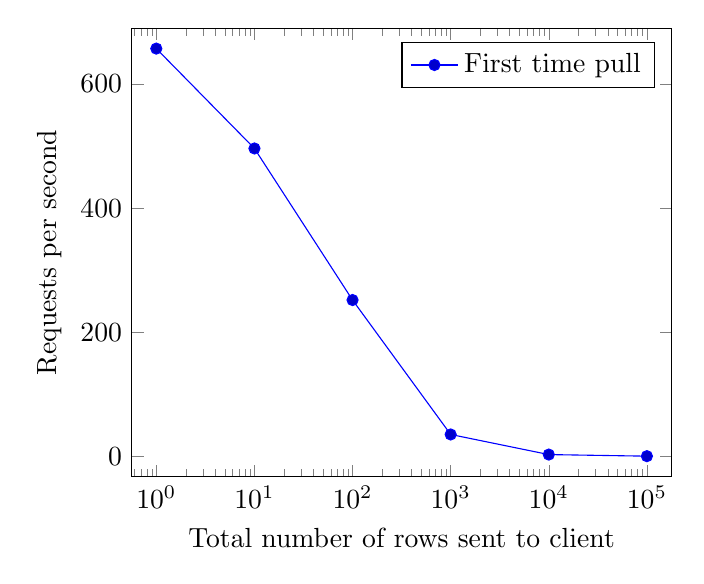
\begin{tikzpicture}
\begin{axis}[
    scaled x ticks=false,
    xticklabel style={
        /pgf/number format/fixed,
    },
    enlargelimits=0.05,
    xmode=log,
    legend pos=north east,
	ylabel=Requests per second,
    xlabel=Total number of rows sent to client,
]
\addplot coordinates {
(1,657.0060383305095)
(10,496.0971386520877)
(100,251.84463804316118)
(1000,35.2212129635721)
(10000,2.8245788253934077)
(100000,0.25184602796491373)
};
\legend{First time pull}
\end{axis}
\end{tikzpicture}

}

    \caption{Throughput in requests per second for the first pull of a new client.}
    \label{fig:server-initial-pull}
\end{subfigure}
\hfill
\begin{subfigure}[b]{0.48\textwidth}
    \centering
    
\resizebox{\textwidth}{!}{
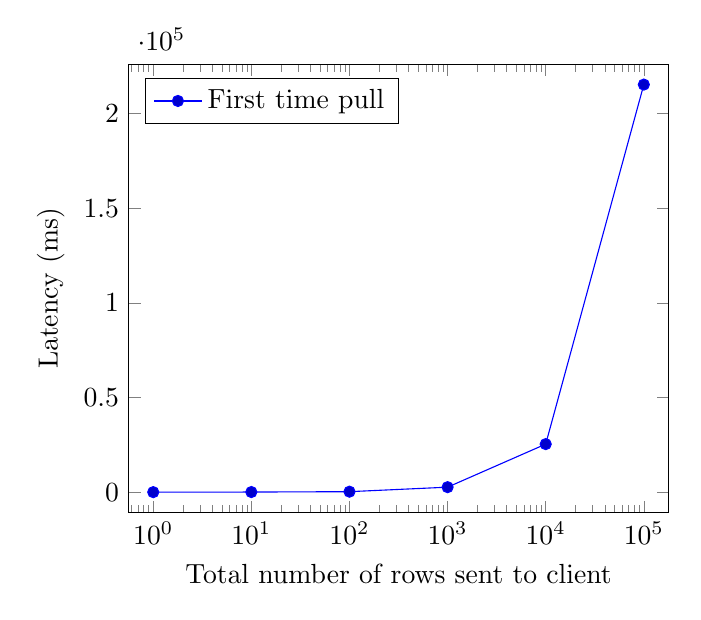
\begin{tikzpicture}
\begin{axis}[
    scaled x ticks=false,
    xticklabel style={
        /pgf/number format/fixed,
    },
    enlargelimits=0.05,
    xmode=log,
    legend pos=north west,
	ylabel=Latency (ms),
    xlabel=Total number of rows sent to client,
]
\addplot coordinates {
(1,151.3177991927478)
(10,200.66596799458623)
(100,394.9383148017856)
(1000,2775.0688378771424)
(10000,25507.10786557448)
(100000,215327.59411900997)
};
\legend{First time pull}
\end{axis}
\end{tikzpicture}

}

    \caption{Latency in milliseconds for the first pull of a new client.}
    \label{fig:server-initial-pull-latency}
\end{subfigure}
\\
\begin{subfigure}[b]{0.48\textwidth}
    \centering
    
\resizebox{\textwidth}{!}{
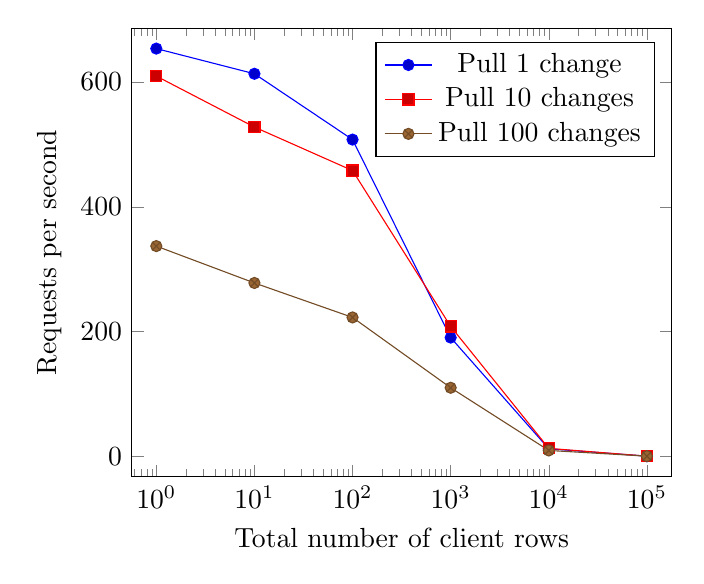
\begin{tikzpicture}
\begin{axis}[
    scaled x ticks=false,
    xticklabel style={
        /pgf/number format/fixed,
    },
    enlargelimits=0.05,
    xmode=log,
    legend pos=north east,
	ylabel=Requests per second,
    xlabel=Total number of client rows,
]
\addplot coordinates {
(1,653.5612346042873)
(10,613.2046001376317)
(100,507.6932618424054)
(1000,190.3224663079544)
(10000,12.073470108310966)
(100000,0.24330810427470806)
};
\addplot coordinates {
(1,609.4821193489477)
(10,527.7649745925163)
(100,458.0218986062899)
(1000,208.2099970380556)
(10000,12.728281373988962)
(100000,0.2301999588809523)
};
\addplot coordinates {
(1,336.9617065960883)
(10,277.88085543440116)
(100,222.6381063149333)
(1000,109.89068215130281)
(10000,9.375860439877298)
(100000,0.24585339309219226)
};
\legend{Pull 1 change,Pull 10 changes,Pull 100 changes}
\end{axis}
\end{tikzpicture}

}

    \caption{Throughput for subsequent pulls of clients for N changed rows.}
    \label{fig:server-pull-n}
\end{subfigure}
\hfill
\begin{subfigure}[b]{0.48\textwidth}
    \centering
    
\resizebox{\textwidth}{!}{
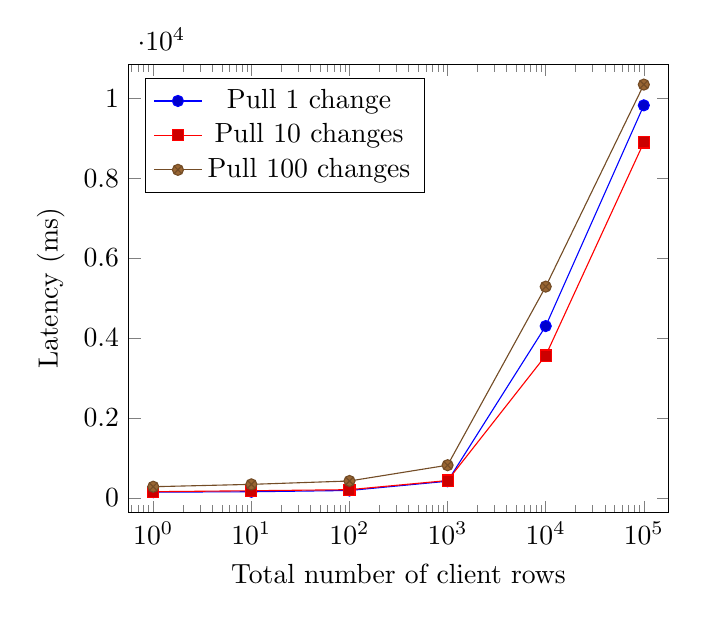
\begin{tikzpicture}
\begin{axis}[
    scaled x ticks=false,
    xticklabel style={
        /pgf/number format/fixed,
    },
    enlargelimits=0.05,
    xmode=log,
    legend pos=north west,
	ylabel=Latency (ms),
    xlabel=Total number of client rows,
]
\addplot coordinates {
(1,148.14735268270476)
(10,157.65048691576123)
(100,189.3937662708464)
(1000,421.2229768074456)
(10000,4299.91606961319)
(100000,9818.9874564031)
};
\addplot coordinates {
(1,158.84961668989848)
(10,183.10149501011867)
(100,209.5507787674066)
(1000,438.027094739863)
(10000,3563.2274893531403)
(100000,8890.628670804876)
};
\addplot coordinates {
(1,283.62712974450164)
(10,342.5796123858848)
(100,426.792526897295)
(1000,821.7966148666502)
(10000,5286.218562150145)
(100000,10337.796716703124)
};
\legend{Pull 1 change,Pull 10 changes,Pull 100 changes}
\end{axis}
\end{tikzpicture}

}

    \caption{Latency in milliseconds for subsequent pulls of clients for N changed rows.}
    \label{fig:server-pull-n-latency}
\end{subfigure}
\\
\begin{subfigure}[b]{0.48\textwidth}
    \centering
    
\resizebox{\textwidth}{!}{
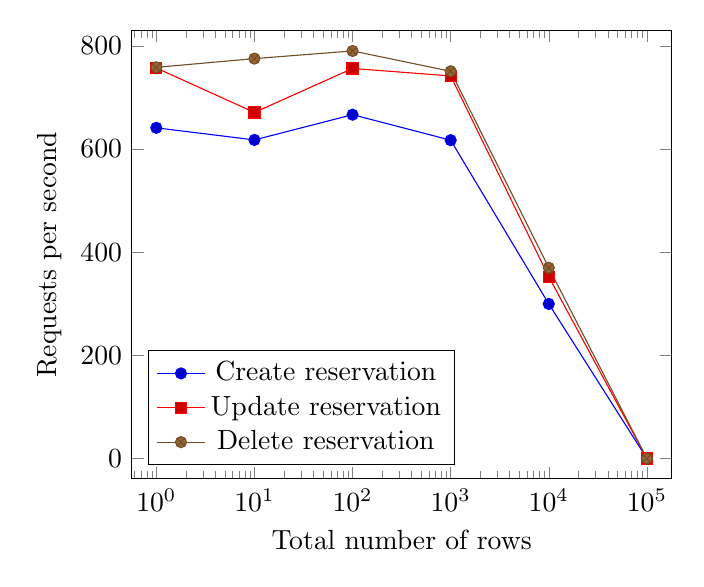
\begin{tikzpicture}
\begin{axis}[
    scaled x ticks=false,
    xticklabel style={
        /pgf/number format/fixed,
    },
    enlargelimits=0.05,
    xmode=log,
    legend pos=south west,
	ylabel=Requests per second,
    xlabel=Total number of rows,
]
\addplot coordinates {
(1,641.0351528906754)
(10,617.6240684602672)
(100,666.5243349523964)
(1000,617.1142287180805)
(10000,299.7614854163515)
(100000,0.23332479590905358)
};
\addplot coordinates {
(1,756.9864665774749)
(10,670.8634485549774)
(100,756.1108375545527)
(1000,741.6174164744328)
(10000,352.3150084321744)
(100000,0.2666610647665712)
};
\addplot coordinates {
(1,758.2312458525041)
(10,775.1915568830312)
(100,790.0564659291424)
(1000,750.6254936296981)
(10000,369.795931154305)
(100000,0.2499978774638541)
};
\legend{Create reservation,Update reservation,Delete reservation}
\end{axis}
\end{tikzpicture}

}

    \caption{Throughput for pushing mutations to the server.}
    \label{fig:server-push}
\end{subfigure}
\hfill
\begin{subfigure}[b]{0.48\textwidth}
    \centering
    
\resizebox{\textwidth}{!}{
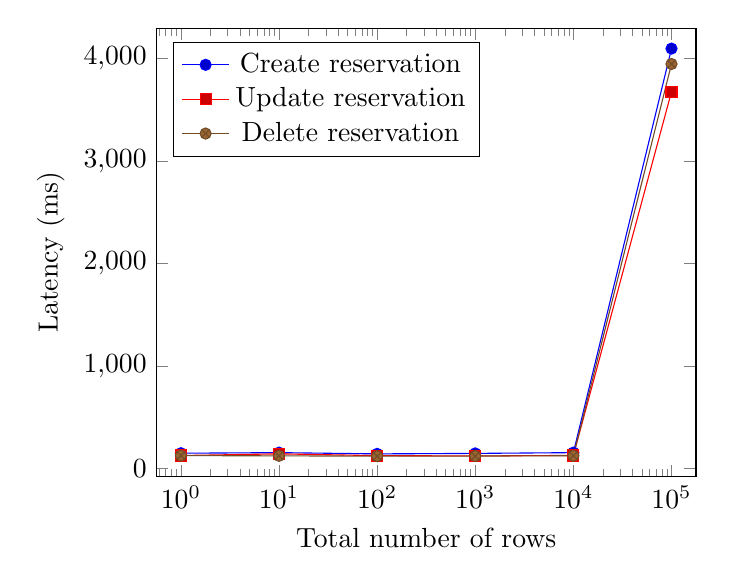
\begin{tikzpicture}
\begin{axis}[
    scaled x ticks=false,
    xticklabel style={
        /pgf/number format/fixed,
    },
    enlargelimits=0.05,
    xmode=log,
    legend pos=north west,
	ylabel=Latency (ms),
    xlabel=Total number of rows,
]
\addplot coordinates {
(1,150.66110655384165)
(10,156.41844166369114)
(100,144.26709320695832)
(1000,148.9411548160028)
(10000,156.43923551236495)
(100000,4097.589489285714)
};
\addplot coordinates {
(1,128.1384544347074)
(10,144.43965793143613)
(100,127.20183198755986)
(1000,124.13043367755586)
(10000,129.2090453631025)
(100000,3676.4989655000004)
};
\addplot coordinates {
(1,127.64813295826666)
(10,125.02174964813253)
(100,122.03751497396983)
(1000,122.97127084164389)
(10000,126.18721079759442)
(100000,3947.563917333334)
};
\legend{Create reservation,Update reservation,Delete reservation}
\end{axis}
\end{tikzpicture}

}

    \caption{Latency in milliseconds for pushing mutations to the server.}
    \label{fig:server-push-latency}
\end{subfigure}
    
    \caption{Throughput of server for handling pull and push requests by total number of rows in client state.}
    \label{fig:server-relic-experiment}
\end{figure}
